\documentclass{IOS-Book-Article}

\usepackage{mathptmx}
\usepackage{amsmath}
\usepackage{color}
\usepackage{tabularx}
\usepackage{booktabs}
\usepackage{mwe}

\makeatletter

\usepackage[utf8]{inputenc}

\usepackage{times}
\normalfont
\usepackage[T1]{fontenc}
%\usepackage[mtplusscr,mtbold]{mathtime}

\usepackage{tikz}
\usepackage{blindtext, graphicx}

\usepackage{enumerate}

\usepackage{float} % allows 'H' positioning tag

% allow use of subfigures
\usepackage{caption}
\usepackage{subcaption}

\usepackage{multirow}
\usepackage{amssymb}
\usepackage{tablefootnote}
\usepackage{hyperref}
\usepackage{epstopdf}

\usepackage{amsmath}

\usepackage{smartdiagram}

\newcommand{\degree}{\ensuremath{^{\circ}}\xspace}


%

\begin{document}
\pagestyle{headings}
\def\thepage{}
\begin{frontmatter}                            % The preamble begins here.

%\pretitle{Pretitle}
\title{Weighted Kappa Loss Function for Ordinal Regression in Deep Learning
%\thanks{...}
}
%\runningtitle{}
%\subtitle{Subtitle}

\author{\fnms{Jordi} \snm{de la Torre}, \fnms{Aida} \snm{Valls}, \fnms{Domenec} \snm{Puig}}

\runningauthor{J. de la Torre et al.}
\address{Departament d'Enginyeria Inform\`{a}tica i Matem\`{a}tiques\\ Universitat Rovira i Virgili, Tarragona}
\email{jordi.delatorre@gmail.com, aida.valls@urv.cat,  domenec.puig@urv.cat}



\begin{abstract}
Weighted Kappa is a index of reference used in many diagnosis systems to compare the agreement between different raters. This index can be also used to compare the goodness of a machine-learning based classification method against the results gotten from a consensus expert group. On the other hand, deep learning has achieved in the last years a great importance as a machine learning method for designing classification algorithms also for medical diagnosis. In this paper we explore the direct use of a Weighted Kappa loss function for the optimization of classification ratings, where one ore more underlying causes induce some pr-established ordering of the classes to predict. We show that for the case of diabetic retinopathy image classification, better results can be obtained from the direct optimization of Kappa over the results obtained from the usage of a multi-class logarithmic loss function.
\end{abstract}

\begin{keyword}
deep learning, convolutional neural networks, supervised learning, computer vision, diabetic retinopathy, cohen's kappa, loss function, ordinal data, weighted kappa, ordinal regression
\end{keyword}
\end{frontmatter}

\thispagestyle{empty}
\pagestyle{empty}

\section{Introduction}

Deep Learning methods have been used extensively in the last years for many automatic classification tasks. The scheme used for images, is based on extracting the important features with a set of convolutional layers and after that make a final classification with them using a set of fully connected layers. A last softmax output layer gives as a result the predicted output probabilities of the set of classes the model. During training the model parameters are changed using a gradient based optimization algorithm, minimizing a predefined loss function. For multi-class classification the standardized loss function used is the logarithmic loss.

\begin{figure}
	\caption{High Level Description of a Deep Learning Image Classification Scheme}
	\centering
	\smartdiagramset{back arrow disabled=true}
	\smartdiagram[flow diagram:horizontal]{Image Input, Feature Extraction Layers, Classification Layers, Class Probability, Cost\\Function}
\end{figure}

On the other hand, many medical diagnosis systems use Quadratic Weighted Kappa Index ($\kappa$) for measuring the level of agreement between raters in such applications where some underlying factors present on images or data need to be interpreted in order to infer from them a diagnose. In this interpretation normally is present some level of subjectivity that make sometimes the conclusions of different experts to differ. Weighted Kappa is able to measure the level of discrepancy of a set of diagnosis made by different raters over the same population. Depending on the value of the index, the strength of agreement between the raters can be evaluated (see table \ref{tab:kappa_int}). 

Examples of the usage of such index are the study of the reliability and distinguish-ability of X-rays films, ultrasounds, retine images, the diagnosis of psychological disorders, between many others. $\kappa$ takes into account the pr-established ordering of the classes and penalizes the erroneous predictions in function of the distance. This index can be used also to measure the goodness of the prediction taken from a machine learning method. The values of the prediction can be compared against the correct values reported by a human experts consensus group. In that way, the index compares the values predicted by the model with the considered "true value" coming from the consensus of a human experts group.


\begin{center}
	\captionof{table}{Table Interpretation of kappa, after Landis and Koch (1977)}
	\label{tab:kappa_int}
	\begin{tabular}{llr}
		\hline
		Kappa    & Strength of agreement \\
		\hline
		<0.20 		& Poor \\
		0.21-0.40 	& Fair \\
		0.41-0.60 	& Moderate \\
		0.61-0.80 	& Good \\
		0.81-1.00 	& Very good \\
		\hline
	\end{tabular}
\end{center}

In this paper, we study the direct optimization of the quadratic weighted kappa ($\kappa$). We use it not only as a evaluation function but also as loss function. We use a diabetic retinopathy image classification problem to compare the performance of the results obtained from the use of the standard logarithmic loss against the results obtained from the optimization of the weighted kappa.

The study is organized as follows: we present the background of this work showing the standardized loss function used for classification, next we propose the new cost function for multi-class classification of ordinal data (ordinal regression) with all the mathematical equations required for the optimization, we define the experiments, the results obtained and finally present the conclusions.

\section{Background}

Deep Learning is a Machine Learning Algorithm used between other tasks for image classification. In the last years this method report the best classification scores for many applications. This image classification methods use a convolutional neural network of different layers for making the automatic feature extraction followed by a one or more classification layers (normally fully connected layers) and a final output layer formed by as many outputs as classes to predict. It is usual to have in such an output layer a softmax function that report as output the probability to belong to every class. Normally, the chosen class is the one that report a higher probability on the output layer. This neural network architecture has many parameters on every layer that have to be optimized to get the most exact probability in the outputs. This is done defining an optimization function in the output, called loss function. This loss function has some dependency on the output probabilities. Calculating the derivatives of such function is possible to apply a gradient descent based algorithm to optimize such a function. The parameters of the network are updated backpropagating the gradient of the function over the network.

The standard loss function used for classification purposes is the logarithmic loss function. This function has been proven to be very effective for the optimization of classification tasks, their derivatives are easy to calculate and has a very robust probabilistic foundation: minimizing the logarithmic loss is the same as minimizing the logarithmic likelihood, that is equivalent to doing a maximum likelihood estimation (MLE) or equivalently, to finding the maximum a posteriori probability (MAP), given a uniform prior. 

As stated above, this logarithmic function does not encode any prior information about the classes. There are cases where there is some sort of previously known relationship between the classes. In those cases, when using the logarithmic loss such a information has to be learned by the network from data. This fact can be a disavantadge when there is not enough data available. A loss that encodes such a prior information can perform better or faster due to the fact that does not require to learn such a information from the data.

This case happens when there is a predefined ordering of the classes based on some sort of previously unknown properties. When doing the classification using the logarithmic loss, such an ordering has to be inferred from data. In this paper we want to explore if there is some advantage in using a different loss function that encodes such a previously known information in the results of the classification.

Supervised deep learning techniques are used extensively for many automatic classification tasks. In the case of images, most of the state of the art methods are based on the use of deep convolutional neural networks (CNN). These techniques are focused on learning multiple levels of representation and abstraction that help to make sense of the hidden information in data such as images. In this way, having a complete set of correctly classified images and without any a priori understanding of the features, the system is able to learn the properties of the image that minimize a defined cost function that is direct or indirectly related with the classification score index to optimize. CNN have proved to be the best available method for solving the biggest classification challenges, like image classification in IMAGENET\cite{ILSVRC15}. 

Multi-class classification is addressed mainly by the use of the logarithmic loss function. This function is very easy to optimize using gradient descent methods due to the simplicity of its derivatives, its numerical stability and experimental tested validity.

\begin{equation*}
\begin{aligned}
\label{eq:log-loss}
&\mathcal{L} = \frac{1}{N} \sum_{i=1}^N \sum_{c=1}^C t_i \log{y_i^{(c)}} \\
\text{where:}\\
&\text{N is the number of samples}\\
&t_i \text{ is 1 for the correct class of sample i and 0 elsewhere}\\
&\text{C is the number of classes}\\
\end{aligned}
\end{equation*}


In the cases where a multi-class classification of ordinal data (ordinal regression) is required, we know in advance prior to the training that the classes have some sort of predefined cardinality. Such information can be of utility for speeding up and improving the classification if can be encoded in the loss function. Logarithmic loss, due to its nature, does not encode such information and has to learn from data such a predefined ordering of the classes.

\section{QWK Loss Function}

Weighted Kappa is an index that measure the inter-rating agreement between a set of different classes where these categories are ordinal in such a way that the property that we want to categorize have some sort of implicit ordering that we want to extract from the categorization. This index establishes a penalization when there is some sort of discrepancy between the ratters that depends from the distance of both predictions. In the case of the Quadratic Weighted Kappa the penalization of the discrepancy grows quadratically with the distance between the two ratings. Is the predicted classes of both raters is the same we say the there is an absolute concordance between both raters and no penalization is applied. When the predicted classes are different, we say that the there is relative concordance between both raters and there is a penalization in the calculation of the inter-rating index that is proportional of the square of the distance between both predictions. This discrepancies are calculated for all the N items of the k mutually exclusive categories and summed over the N items. The penalizing term is normalized dividing their value by the expected  discrepancy, obtaining as a result a value between -1 and 1. A value of 1 of the index would indicate a perfect agreement between both raters, -1 a perfect symmetric disagreement between the classes and 0 a random evaluation method. 

\subsection{Mathematical Foundation}

The Kappa function can be written as:

\begin{equation*}
\begin{aligned}
&\kappa = 1 - \frac{ \sum_{i,j} \omega_{i,j} O_{i,j} }
{\sum_{i,j} \omega_{i,j} E_{i,j}}\\
\text{where:}\\
&\text{C is the number of classes}\\
&\omega_{i,j} = \frac{(i-j)^n}{(C - 1)^n}\\
&\text{i, j} \in \{ 1, 2, ..., C\}\\
\end{aligned}
\end{equation*}

For the case of the Quadratic Weighted Kappa, n = 2.

For the case of the QWK loss function, the optimization algorithm to solve is the next:

\begin{equation*}
\begin{aligned}
& \underset{x}{\text{maximize}}
& & \kappa = 1 - \frac{ \sum_{i,j} \omega_{i,j} O_{i,j} }
{\sum_{i,j} \omega_{i,j} E_{i,j}} & & \kappa \in [-1,1]\\
\end{aligned}
\end{equation*}

That is the same as:

\begin{equation*}
\begin{aligned}
& \underset{x}{\text{minimize}}
& & \mathcal{L} = \log{\left( 1 - \kappa \right)} = \log{\left( \frac{ \sum_{i,j} \omega_{i,j} O_{i,j} }{\sum_{i,j} \omega_{i,j} E_{i,j}} \right) } = \log{\left(\frac{\{Num\}}{\{Den\}}\right)} & & \mathcal{L} \in \left(-\infty,0\right]
\end{aligned}
\end{equation*}

\begin{equation*}
\begin{aligned}
& \{ Num \} = \sum_{i,j} \omega_{i,j} O_{i,j} = \sum_{k=1}^N \sum_{c=1}^C \omega_{t_k,c}^{(k)} P_c^{(k)} = \sum_{k=1}^N \sum_{c=1}^C \omega_{t_k,c}^{(k)} y_c^{(k)}\\
&\{ Den \} = \sum_{i,j} \omega_{i,j} E_{i,j} = \sum_{i=1}^C \sum_{j=1}^C \omega_{i,j} \hat{N_i} \sum_{k=1}^N y_j^{(k)} = \sum_{i=1}^C \hat{N_i} \sum_{j=1}^C \left( \omega_{i,j} \sum_{k=1}^N y_j^{(k)}\right)\\
& E_{i,j} = \frac{N_i \sum_{k=1}^N P_j^{(k)}}{N} = = \hat{N_i} \sum_{k=1}^N P_j^{(k)}
\end{aligned}
\end{equation*}

where:

N: number of samples

$N_i$: number of samples of class i

$\hat{N_i}$ = $\frac{N_i}{N}$

$t_k$: correct class number for sample k

$P_c^{(k)}$: probability that sample k is of class C given that the true class in $t_k$

$y_c^{(k)}$: probability given by the model. In our case $y_c^{(k)}$ = $P_c^{(k)}$

\subsection{Partial Derivatives of the QWK Derived Loss Function}

For solving this optimization problem using any gradient descent based algorithm, we need to derive the partial derivatives of the loss function with respect to the output variables of the network. 

For the case minimizing the loss function $\mathcal{L} =\log{ \frac{\{Num\}}{\{Den\}}}$, the derivative takes the next form:

\begin{equation*}
\begin{aligned}
\frac{\partial \mathcal{L}}{\partial y_m} = \frac{1}{\{Num\}}\frac{\partial \{Num\}}{\partial y_m} - \frac{1}{\{Den\}}
\frac{\partial{\{Den\}}}{\partial y_m}
\end{aligned}
\end{equation*}

And $\frac{\partial \{Num\}}{\partial y_m}$ and $\frac{\partial{\{Den\}}}{\partial y_m}$ can be calculated with the next expressions:

\begin{equation*}
\begin{aligned}
& \frac{\partial \{ Num\}}{\partial y_m^{(k)}} = \omega_{t_k m}^{(k)} & \frac{\partial \{ Den\}}{\partial y_m^{(k)}} = \sum_{i=1}^{C} \hat{N_i} \omega_{i,m}\\
& m \in \{1, 2, ..., C\}
\end{aligned}
\end{equation*}

That in its array form can be rewritten as:


\begin{equation*}
\begin{aligned}
\frac{\partial \{ Num\}}{\partial y_m} =
\begin{pmatrix} 
	\omega_{t_1, 1}     & \omega_{t_1, 2}     & ...     & ... & \omega_{t_1, C}\\ 
	\omega_{t_2, 1}     & \omega_{t_2, 2}     & ...     & ... & \omega_{t_2, C}\\ 
	...					& ...		          & ...     & ... & ...\\
	\omega_{t_N, 1}     & \omega_{t_N, 2}     & ...     & ... & \omega_{t_N, C}\\  
\end{pmatrix}
\end{aligned}
\end{equation*}

\begin{equation*}
\begin{aligned}
\frac{\partial \{ Den\}}{\partial y_m} =
\begin{pmatrix} 
\sum_{i=1}^C \hat{N_i} \omega_{1,i} & ...  & ...     & ... & \sum_{i=1}^C \hat{N_i} \omega_{C,i}\\
\sum_{i=1}^C \hat{N_i} \omega_{1,i} & ...  & ...     & ... & \sum_{i=1}^C \hat{N_i} \omega_{C,i}\\
... & ::: & ... & ... & ...\\
\sum_{i=1}^C \hat{N_i} \omega_{1,i} & ...  & ...     & ... & \sum_{i=1}^C \hat{N_i} \omega_{C,i}\\ 
\end{pmatrix}
\end{aligned}
\end{equation*}


\section{Experiments}


The objective of the experiments is to study the differences between the optimization of two different loss functions in order to evaluate how the $\kappa$ loss function performs in comparison with the standard multiclass classification logarithmic loss function. In order to make the comparison possible a unique deep network architecture will be optimized with both functions. 

As deep learning is a computer intensive task, the experiments have been done using different input resolution images: 128x128, 256x256 and 384x384. The smaller images allow to run more experiments and serve to not only make a first validation of the new cost function but also to make a first hyper-parameters selection that can serve later on to validate the new cost function against higher resolution images using less time consuming experiments.

The dataset used in this work consists of a set of retine images taken with mydriatic camera. All the images are classified by ophthalmologists according to a standardized severity scale \cite{diaclass}. The objective of the training will be to optimize the network with the data available to perform the best in the never seen before test set.

The training set contains a total of 35.126 images; 25.810 of class 0, 2.443 of class 1, 5.292 of class 3, 873 of class 3 and 708 of class 4. The test set contains a total of 53.576 images; 39.533 of class 0, 3.762 of class 1, 7.861 of class 2, 1.214 of class 3 and 1.206 of class 4. Notice that both sets are highly imbalanced.

The original training set is splitted in two random subsets: one with 90\% of the data and other with 10\%. The last one is used as a validation set for hyper-parameter selection. The value of $\kappa$ is calculated every epoch either for the training or the validation set. In all models a ReLU\cite{Dahl2013} activation function is used. In all layers a batch normalization \cite{batch-norm} is applied before the activation function in order to reduce the gradient vanishing problem that occurs in deep networks. A random initialization based in the Kaiming\&He approach\cite{kaiming} is used for all the networks. All models are optimized using Adam over batches. 

We study different learning rates in order to find the optimal one for each loss function. We use a batch-based optimization algorithm. $\kappa$ loss function uses a normalization term that normalizes over the sample set. Presumably this loss function has to be more sensible to small batches that the logarithmic loss due to this normalization term, that's why different batch sizes are tested. For every batch, the images are chosen randomly from the training set, with repetition. Data augmentation techniques are applied to augment the diversity of the classes (random rotations and brigthness and contrast modifications). The epoch size is set to maintain fixed the total number of images per epoch to 100.000. This value is approximately the number of images required to sample to ensure that all of them has been selected every epoch. Also, using different batch sizes, the number of updates per epoch of the parameters of the neural network change. In the case of small batch sizes the number of updates per epoch is greater than the case of big batch sizes. Studying different batch sizes we would also explore different number of parameter updates.

\begin{table}[h!]
	\centering
	\caption{Neural network architecture used in the experiments}
	\label{tab:nn}
	\begin{tabular}{l|c|l|r}
		Layer & N & Type & Size \\
		\hline
		0 & 0 & Input & 3x128x128\\
		\hline
		\multirow{3}{*}{1} & 1 & Convolution:3x3 Padding:1,1 Step:1,1 Channels:3->32 & \multirow{6}{*}{32x128x128}\\
		& 2 & Batch normalization &\\
		& 3 & ReLU & \\\cline{1-3}
		\multirow{3}{*}{2} & 4 & Convolution:3x3 Padding:1,1 Step:1,1 Channels:32->32 &\\
		& 5 & Batch normalization &\\
		& 6 & ReLU & \\
		& 7 & Max pooling: 2,2 Step: 2,2\\
		\hline
		\multirow{3}{*}{3} & 8 & Convolution:3x3 Padding:1,1 Step:1,1 Channels:32->64 & \multirow{6}{*}{64x64x64}\\
		& 9 & Batch normalization &\\
		& 10 & ReLU & \\\cline{1-3}
		\multirow{3}{*}{4} & 11 & Convolution:3x3 Padding:1,1 Step:1,1 Channels:64->64 &\\
		& 12 & Batch normalization &\\
		& 13 & ReLU & \\
		& 14 & Max pooling: 2,2 Step: 2,2\\
		\hline		 
		\multirow{3}{*}{5} & 15 & Convolution:3x3 Padding:1,1 Step:1,1 Channels:64->128 & \multirow{6}{*}{128x32x32}\\
		& 16 & Batch normalization &\\
		& 17 & ReLU & \\\cline{1-3}
		\multirow{3}{*}{6} & 18 & Convolution:3x3 Padding:1,1 Step:1,1 Channels:128->128 &\\
		& 19 & Batch normalization &\\
		& 20 & ReLU & \\
		& 21 & Max pooling: 2,2 Step: 2,2\\
		\hline
		\multirow{3}{*}{7} & 22 & Convolution:3x3 Padding:1,1 Step:1,1 Channels:128->128 & \multirow{6}{*}{128x16x16}\\
		& 23 & Batch normalization &\\
		& 24 & ReLU & \\\cline{1-3}
		\multirow{3}{*}{8} & 25 & Convolution:3x3 Padding:1,1 Step:1,1 Channels:128->128 &\\
		& 26 & Batch normalization &\\
		& 27 & ReLU & \\
		& 28 & Max pooling: 2,2 Step: 2,2\\
		\hline		
		\multirow{3}{*}{9} & 29 & Convolution:3x3 Padding:1,1 Step:1,1 Channels:128->128 & \multirow{6}{*}{128x8x8}\\
		& 30 & Batch normalization &\\
		& 31 & ReLU & \\\cline{1-3}
		\multirow{3}{*}{10} & 32 & Convolution:3x3 Padding:1,1 Step:1,1 Channels:128->128 &\\
		& 33 & Batch normalization &\\
		& 34 & ReLU & \\
		& 35 & Max pooling: 2,2 Step: 2,2\\
		\hline
	    11 & 36 & Convolution:4x4 Padding:1,1 Step:1,1 Channels:128->128 & 128\\
		\hline
		\multirow{3}{*}{12} & 37 & Linear fully connected & \multirow{3}{*}{128}\\					
		& 38 & Batch normalization &\\
		& 39 & ReLU & \\
		\hline
		\multirow{2}{*}{13} & 40 & Linear fully connected & \multirow{2}{*}{5}\\
		& 41 & Softmax &\\
		\hline
	\end{tabular}
\end{table}


\section{Results}

Table \ref{tab:qwk_cv} shows all the experiments that have been done using both losses using different learning rates and batch sizes. $\kappa$ score is calculated over the cross validation set for comparison between the results obtained from the direct optimization of the function and the standardized indirect method of using the log-loss function. In figure \ref{fig:best} we show a graphical representation of the same results of the table. Here we see that only with very small batch sizes log-loss results perform better than $\kappa$. Probably this is due to the fact that $\kappa$ uses a normalization term in the denominator that in cases were the batch is not big enough causes instabilities in the gradient that affect the performance. In any case, even in those cases the results obtained with the log loss are worse that those achieved using the best $\kappa$ configuration.

\begin{figure}[!htb]
	\centering
	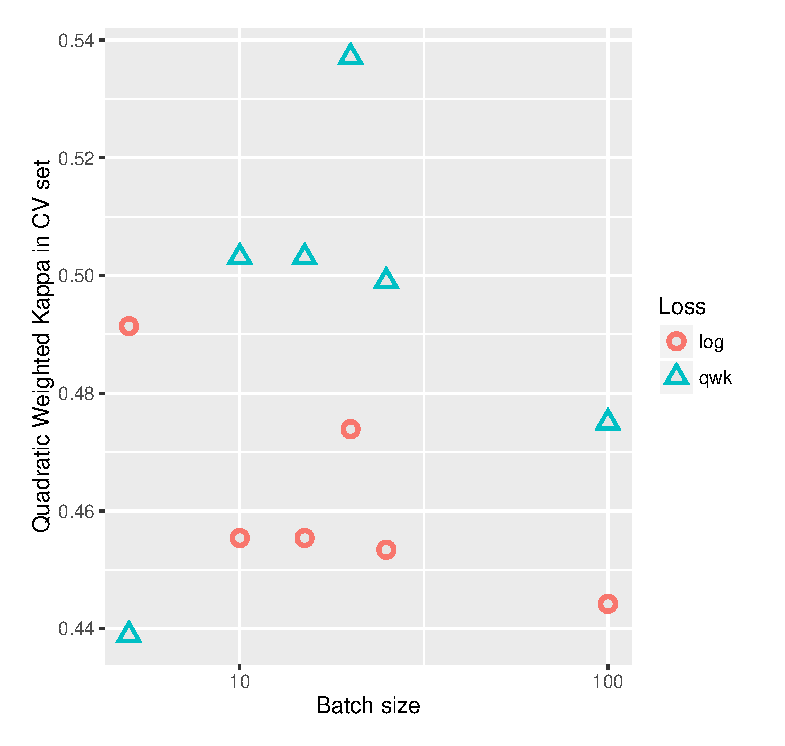
\includegraphics[scale=.7]{best.eps}
	\caption{Best classification results achieved over cross validation set for each loss function}
	\label{fig:best}
\end{figure}


\begin{table}[h!]
	\centering
	\caption{Results achieved in different experiments}
	\label{tab:qwk_cv}
	\begin{tabular}{c|c|c|c|c|c|c|c|c|c|c}
		Input & BS & Loss & LR	& $\kappa_{train} 10^3$ & $\kappa_{test} 10^3$ & Gap & Epoch & Updates $10^{-3}$ & TAG\\	
		\hline
		\multirow{32}{*}{128} & \multirow{6}{*}{5} & \multirow{3}{*}{log} & $10^{-5}$ & 771 & 418 & 353 & 78 & 1560 & E26\\
		& & & $10^{-4}$ & 851 & \textbf{491} & 360 & 73 & 1460 & E24\\
		& & & $10^{-3}$ & 676 & 418 & 258 & 29 & 580 & E25\\\cline{3-10}
		& & \multirow{3}{*}{qwk} & $5 \times 10^{-5}$ & 545 & 402 & 143 & 50 & 1000 & E05\\
		& & & $10^{-5}$ & 646 & 439 & 207 & 70 & 1400 & E31\\
		& & & $10^{-4}$ & 497 & 326 & 171 & 31 & 620 & E04\\
		\cline{2-10}
		&\multirow{6}{*}{10} & \multirow{3}{*}{log} & $10^{-5}$ & 797 & 397 & 400 & 82 & 820 & E08\\
		& & & $10^{-4}$ & 874 & 455 & 419 & 81 & 810 & E07\\
		& & & $10^{-3}$ & 514 & 336 & 178 & 57 & 570 & E01\\\cline{3-10}
		& & \multirow{3}{*}{qwk} &  $10^{-5}$ & 774 & 476 & 298 & 82 & 820 & E12\\
		& & & $10^{-4}$ & 755 & 503 & 252 & 84 & 840 & E02\\
		& & & $10^{-3}$ & 596 & 289 & 307 & 95 & 950 & E06\\
		\cline{2-10}		
		& \multirow{6}{*}{15} & \multirow{3}{*}{log} & $10^{-5}$ & 803 & 368 & 435 & 79 & 527 & E23\\
		& & & $10^{-4}$ & 899 & 458 & 441 & 95 & 633 & E22\\
		& & & $10^{-3}$ & 868 & 447 & 421 & 80 & 533 & E21\\\cline{3-10}
		& & \multirow{3}{*}{qwk} & $5\times10^{-5}$ & 715 & 491 & 224 & 77 & 513 & E14\\
		& & & $10^{-4}$ & 783 & 509 & 274 & 62 & 413 & E15\\
		& & & $5\times10^{-4}$ & 823 & 523 & 300 & 72 & 480 & E16\\
		\cline{2-10}
		& \multirow{2}{*}{20} & log & $10^{-4}$ & 896 & 474 & 422 & 79 & 395 & E35\\\cline{3-10}
		& & qwk & $10^{-4}$ & 835 & \textbf{537} & 298 & 93 & 465 & E34\\
		\cline{2-10}
		& \multirow{6}{*}{25} & \multirow{3}{*}{log} & $10^{-5}$ & 821 & 315 & 506 & 96 & 384 & E28\\
		& & & $10^{-4}$ & 913 & 453 & 460 & 93 & 372 & E27\\
		& & & $10^{-3}$ & 849 & 382 & 467 & 70 & 280 & E33\\\cline{3-10}
		& & \multirow{3}{*}{qwk} & $10^{-5}$ & 808 & 423 & 385 & 95 & 380 & E18\\
		& & & $10^{-4}$ & 824 & 499 & 325 & 65 & 260 & E17\\
		& & & $10^{-3}$ & 655 & 447 & 208 & 80 & 320 & E30\\
		\cline{2-10}
		& \multirow{2}{*}{100} & \multirow{3}{*}{log} & $10^{-4}$ & 929 & 377 & 552 & 98 & 98 & E20\\
		& & & $10^{-3}$ & 947 & 444 & 503 & 99 & 99 & E09\\
		& & & $10^{-2}$ & 842 & 412 & 430 & 67 & 67 & E13\\\cline{3-10}
		& & \multirow{3}{*}{qwk} & $10^{-4}$ & 879 & 450 & 429 & 93 & 93 & E11\\
		& & & $10^{-3}$ & 798 & 455 & 343 & 71 & 71 & E03\\
		& & & $10^{-2}$ & - & - & - & - & - & E32\\
		\hline	
		\multirow{10}{*}{256} & \multirow{2}{*}{5} & \multirow{1}{*}{log} & $10^{-4}$ & 871 & \textbf{571} & 300 & 52 & 1040 & \\\cline{3-10}
		& & \multirow{1}{*}{qwk} & $10^{-4}$ & 605 & 433 & 172 & 15 & 300 & \\
		\cline{2-10}
		&\multirow{2}{*}{10} & \multirow{1}{*}{log} & $10^{-4}$ & 903 & 566  & 337 & 75 & 750 & \\\cline{3-10}
		& & \multirow{1}{*}{qwk} & $10^{-4}$ & 832 & 616 & 216 & 70 & 700 & \\
		\cline{2-10}		
		& \multirow{2}{*}{15} & \multirow{1}{*}{log} & $10^{-4}$ & 925 & 556 & 369 & 98 & 653 & \\\cline{3-10}
		& & \multirow{1}{*}{qwk} & $10^{-4}$ & 878 & \textbf{622} & 256 & 93 & 620 & \\
		\cline{2-10}
		& \multirow{2}{*}{20} & \multirow{1}{*}{log} & $10^{-4}$ & 923 & 525 & 398 & 97 & 485 & \\\cline{3-10}
		& & \multirow{1}{*}{qwk} & $10^{-4}$ &  & \textbf{} &  &  &  & \\
		\cline{2-10}		
		& \multirow{2}{*}{30} & \multirow{1}{*}{log} & $10^{-4}$ & 925 & 514 & 411 & 93 & 310 & \\\cline{3-10}
		& & \multirow{1}{*}{qwk} & $10^{-4}$ & 900 & 586 & 314 & 98 & 327 & \\
		\cline{2-10}
		& \multirow{2}{*}{40} & \multirow{1}{*}{log} & $10^{-4}$ & 922 & 464 & 458 & 93 & 233 & \\\cline{3-10}
		& & \multirow{1}{*}{qwk} & $10^{-4}$ & 894 & 592 & 302 & 78 & 195 & \\
		\cline{2-10}
		\hline					
		\multirow{2}{*}{512} & \multirow{2}{*}{15} & \multirow{1}{*}{log} & $10^{-4}$ &  & 695 &  &  & & \\\cline{3-10}
	    &  & \multirow{1}{*}{qwk} & $10^{-4}$ &  & 717 &  &  & &  \\	
		\cline{2-10}	
		\hline
	\end{tabular}
\end{table}


\section{Conclusions}
In this paper we studied the performance of a diabetic retinopathy model using two different loss functions: the standard logarithmic loss and a new quadratic weighted kappa loss. In the case of willing to optimize the result of quadratic weighted kappa we have shown that is better to optimize directly this function than using the standard way of multiclass classification. QWK loss function encodes the prior information that we have about the classes, that is to say, the predefined ordering of the categorical classes. Logarithmic loss has to learn this ordering from data and this comes to be a disadvantage. Results showed that up to 5\% of increment of QWK scores can be obtained from the direct optimization of the function.


\section*{Acknowledgments}
{\tiny This work is supported by the URV grant 2014PFR-URV-B2-60 and the Spanish research projects PI15/01150 and PI12/01535 (Instituto de Salud Carlos III). The authors would like to thank to the California Healthcare Foundation and EyePACS for providing the images used in this study.}


%\begin{thebibliography}{99}
%\printbibliography
\bibliographystyle{unsrt}
\bibliography{retinopathy}
%\end{thebibliography}
\end{document}

